\documentclass[11pt,a4wide]{article}
\usepackage{verbatim}
\usepackage{listings}
\usepackage{graphicx}
\usepackage{a4wide}
\usepackage{color}
\usepackage{amsmath}
\usepackage{amssymb}
\usepackage[dvips]{epsfig}
\usepackage[T1]{fontenc}
\usepackage{cite} % [2,3,4] --> [2--4]
\usepackage{shadow}
\usepackage{hyperref}
\usepackage{graphicx}
\usepackage[english]{babel}
\usepackage{float}
\usepackage{import}
\setcounter{tocdepth}{2}
\lstset{language=c++}
\lstset{basicstyle=\small}
\lstset{backgroundcolor=\color{white}}
\lstset{frame=single}
\lstset{stringstyle=\ttfamily}
\lstset{keywordstyle=\color{red}\bfseries}
\lstset{commentstyle=\itshape\color{blue}}
\lstset{showspaces=false}
\lstset{showstringspaces=false}
\lstset{showtabs=false}
\lstset{breaklines}
\begin{document}

\title{Physics 905-Computational Physics\break Project 1}
\author{Crispin Contreras}
\date{\today}
\maketitle


\begin{abstract}
This paper discusses the numerical solution to Poisson's equation which is solved in
one dimension and with Dirichlet boundary conditions. The second derivative
is approximated with the three point formula and the equations are discretized.
From this a set of linear equations are obtained and are solved to get the solution.
Two different methods were implemented to solve the set of linear equations. One was a simplified version of Gaussian elimination and the other was using LU decomposition. The two methods were compared by the computation time and the number of floating point operations.
\end{abstract}



\section{Introduction}
We begin with the Poisson's equation in three dimensions  with a known source. After some manipulation we get it to look like a simple second order ordinary differential equation. The second derivative of the equation is approximated by the three point formula and we obtain a set of linear equations. We put them in matrix form which gives us the equation  $\ {\bf A}{\bf v} = \tilde{{\bf b}}$. By writing it in this form we find that $\ {\bf A}$ is a tridiagonal matrix and this leads us to develop a simplified algorithm for Gaussian elimination. The algorithm is implemented in C++ and we look at different sizes of the triadiagonal matrix such as 10, 100, and 1000 which correspond to the step size. I then  compute the relative error for the different sizes and record the time that it takes to carry out the algorithm. I compare these parameters with the LU decomposition which I use from the armadillo library and solve the linear equations with lapack. I also compare the number of floating point operations.


\section{Theory}
We start with Poisson's equation in three dimensions, it reads
\[
\nabla^2 \Phi = -4\pi \rho ({\bf r}).
\]
With a spherically symmetric $\Phi$ and $\rho ({\bf r})$  the equations
simplifies to a one-dimensional equation in $r$, namely
\[
\frac{1}{r^2}\frac{d}{dr}\left(r^2\frac{d\Phi}{dr}\right) = -4\pi \rho(r),
\]
which can be rewritten via a substitution $\Phi(r)= \phi(r)/r$ as
\[
\frac{d^2\phi}{dr^2}= -4\pi r\rho(r).
\]
The inhomogeneous term $f$ or source term is given by the charge distribution $\rho$  multiplied by $r$ and the constant $-4\pi$. We will rewrite this equation by letting $\phi\rightarrow u$ and 
$r\rightarrow x$. The general one-dimensional Poisson equation reads then $\-u''(x) = f(x).$
We then solve the one dimensional Poisson's Equation with Dirichlet boundary conditions by rewriting it as a set of linear equations.
To be more explicit we will solve the equation
\[
-u''(x) = f(x), \hspace{0.5cm} x\in(0,1), \hspace{0.5cm} u(0) = u(1) = 0.
\]
and we define the discretized approximation  to $u$ as $v_i$  with 
grid points $x_i=ih$   in the interval from $x_0=0$ to $x_{n+1}=1$.
The step length or spacing is defined as $h=1/(n+1)$. 
We have then the boundary conditions $v_0 = v_{n+1} = 0$.
We  approximate the second derivative of $u$ with the three point formula
\begin{equation}
   -\frac{v_{i+1}+v_{i-1}-2v_i}{h^2} = f_i  \hspace{0.5cm}    
   \mathrm{for} \hspace{0.1cm} i=1,\dots, n, 
\end{equation}
where $f_i=f(x_i)$. Rewriting equation (1) with indeces we have 
\begin{equation}
	-v_{(i)(i+1)}-v_{(i+1)(i)}+2v_{ii}= {f_i}{h^2}
\end{equation}
and set any of the indeces i that are greater than n to zero. These equations lead to the form
\begin{equation}
   {\bf A}{\bf v} = \tilde{{\bf b}},
\end{equation}
where ${\bf A}$ is an $n\times n$  tridiagonal matrix which we rewrite as 
\begin{equation}
    {\bf A} = \left(\begin{array}{ccccccc}
                           2& -1& 0& \dots& \dots&  \dots &0 \\
                           -1 & 2 & -1 &0 &\dots &\dots &0 \\
                           0&-1 &2 & -1 & 0 & \dots &0\\
                           \dots& \dots   & \dots &\dots   &\dots & \dots &\dots\\
                           
						  \dots &\dots &\dots &\dots &\dots &\dots &\dots \\
                           0 &\dots   &\dots  &\dots &-1 &2& -1 \\
                           0 &\dots    &\dots  &\dots & 0  &-1 & 2 \\
                      \end{array} \right)
\end{equation}
and $\tilde{b}_i=h^2f_i$.


In our case we will assume  that the source term is 
$f(x) = 100e^{-10x}$, and keep the same interval and boundary 
conditions. Then the above differential equation
has a closed-form  solution given by $u(x) = 1-(1-e^{-10})x-e^{-10x}$. 

\section{Methods}
Two methods were implemented to solve this equation. One which follows from theory 
section and is similar to Gaussian elimination and the other is using LU decomposition.

\subsection{Method 1: Gaussian Elimination}
From equation (2) we set up the set of linear equations. I started by looking at a 4 by 
4 matrix and used forward substitution and backward substitution to obtain the solutions. By looking at a 4 by 4 matrix and using forward and backward substitution I noticed a pattern which comes from the fact that our matrix is tridiagonal. I start with a general 4 by 4 matrix 

\begin{equation}
\left[\begin{array}{cccc|c}
                           d_1& e& 0& 0& b_1\\ 
                           e& d_2& e& 0& b_2\\
                           0& e& d_3& e& b_3\\
                           0& 0& e& d_4& b_4\\
                      \end{array} \right]
\end{equation}
and for simplicity set all the off diagonal terms to e since in our matrix they are all equal to -1. I 
multiply the first row by $e/d_1$ and subtract from the second row to obtain 

\begin{equation}
\left[\begin{array}{cccc|c}
                           d_1& e& 0& 0& b_1\\ 
                           0& \tilde{d}_2& e& 0& \tilde{b}_2\\
                           0& e& d_3& e& b_3\\
                           0& 0& e& d_4& b_4\\
                      \end{array} \right]
\end{equation}
I then multiply the second row by $e/\tilde{d}_2$ and subtract it from the third row. Finally I multiply
the third row by $e/\tilde{d}_3$ and subtract it from the fourth row. I finally obtain the following matrix
\begin{equation}
\left[\begin{array}{cccc|c}
                           d_1& e& 0& 0& b_1\\ 
                           0& \tilde{d}_2& e& 0& \tilde{b}_2\\
                           0& 0& \tilde{d}_3& e& \tilde{b}_3\\
                           0& 0& 0& \tilde{d}_4& \tilde{b}_4\\
                      \end{array} \right]
\end{equation}
The first row is unchanged and I obtain the equations 
\begin{equation}
\begin{split}
 	\tilde{d}_2 =d_2 - \frac{e}{d_1} \hspace{0.5cm} \tilde{d}_3 =d_3 -\frac{e}{\tilde{d}_2} \hspace{0.5cm} \tilde{d}_4 = d_4 -\frac{e}{\tilde{d}_3} \\
 	\tilde{b}_2 =b_2 -\frac{e}{d_1}b_1 \hspace{0.5cm} \tilde{b}_3 =b_3 -\frac{e}{\tilde{d}_2}\tilde{b}_2 \hspace{0.5cm} \tilde{b}_4 =b_4 -\frac{e}{\tilde{d}_3}\tilde{b}_3
\end{split}
\end{equation}
It's clear to see from these equations the following pattern
\begin{equation}
 	\tilde{d}_i =d_i + \frac{1}{\tilde{d}_i} \hspace{0.5cm}  \tilde{b}_i =b_i +\frac{1}{\tilde{d}_{i-1}}\tilde{b}_{i-1}
\end{equation}
where I have put in the value for e which is equal to -1 and changed $d_1$ to $\tilde{d}_1$ and similarly for b. From equations (7)
and (3) I then obtain the following solutions for v which is done by backward substitution
\begin{equation}
 	v_4 =\frac{\tilde{b}_4}{\tilde{d}_4} \hspace{0.5cm} v_3 =\frac{\tilde{b}_3 -ev_4}{\tilde{d}_3} \hspace{0.5cm} 			  
	v_2=\frac{\tilde{b}_2 -ev_3}{\tilde{d}_2} \hspace{0.5cm} v_1 =\frac{\tilde{b}_1 -ev_2}{\tilde{d}_1}
\end{equation}
For these I also obtain a general formula which holds for i less than 4
\begin{equation}
	v_i =\frac{\tilde{b}_i + v_{i+1}}{\tilde{d}_i}
\end{equation}
where again I put in the value for for e. In C++ I implemented the forward and backward substitution this way 
 
\begin{lstlisting}[title={Project1}]
        //FORWARD SUBSTITUTION
        diagonal_element[0] = 2.0; // Defines First Diagonal element    
        for(int i=0; i <= ( size_matrix+1); i++)
        {
                //Calculate diagonal terms
                if(i < size_matrix)
                {
                        diagonal_element[i+1] = 2.0-(1.0/diagonal_element[i]);

                }//end if statement


                //Calculate known functions
                if( (i>0) && (i<size_matrix))
                {
                        known_fun[i] += known_fun[i-1]/diagonal_element[i-1] ;

                }


        }//End of Loop
        
        //BACKWARD SUBSTITUTION 
        numerical_f[size_matrix]= known_fun[size_matrix-1]/diagonal_element[size_matrix -1];
        numerical_f[0]=0.0;
        numerical_f[size_matrix+1]=0;


        for(int m = (size_matrix-1); m > 0; m-- )
        {
                        numerical_f[m] = (known_fun[m-1] + numerical_f[m+1])/diagonal_element[m-1];

        }//End of Loop
\end{lstlisting}
\begin{center}
Listing 1: This shows sample code to calculate the forward and backward substitution.
\end{center}

These algorithms solve the equations and give the solution $v_i$. The number of floating point operations are counted by how many +, -, *, and / are in the equations. For the forward substitution there are a total of 4 and $(n-1)$ equations to solve and for the backward substitution there are $2(n-1)$. This give us a total of $6(n-1)$ floating point operations which is of the order of $\mathcal{O}(6n)$. Comparing this to the full Gaussian elimination which is given by $\frac{2}{3}n^3 +\mathcal{O}(n^2)$ [1] we see that our method is much faster. 

\subsection{Method 2: LU Decomposition}
We start with equation (3) and decompose  ${\bf A}$ into a lower triangular matrix ${\bf L}$ and an upper triangular matrix ${\bf U}$. This gives 
\begin{equation}
 A = \left[\begin{array}{cccccc}
                           1& 0& 0& \dots& \dots& 0\\ 
                           l_{21}& 1& 0& \dots& \dots& 0\\
                           l_{31}& l_{32}& 1& 0& \dots& 0\\   
                           \vdots& \vdots& \vdots& \ddots& \vdots& \vdots\\                        
                           \vdots& \vdots& \vdots& \vdots& \ddots& \vdots\\
                           l_{n1}& l_{n2}& l_{n3}& \dots& \dots& 1\\
                      \end{array} \right]                      
   \left[\begin{array}{cccccc}
                           u_{11}& u_{12}& u_{13}& \dots& \dots& u_{1n}\\ 
                           0& u_{22}& u_{23}& \dots& \dots& u_{2n}\\
                           0& 0& u_{33}& u_{34}& \dots& u_{3n}\\   
                           \vdots& \vdots& 0& \ddots& \vdots& \vdots\\                        
                           \vdots& \vdots& \vdots& 0& \ddots& \vdots\\
                           0& 0& 0& 0& \dots& u_{nn}\\
                      \end{array}\right]
\end{equation}
We can now rewrite (3) as ${\bf L}({\bf U}{\bf v})= \tilde{{\bf b}}$ and this leads to two equations 
\begin{equation}
 {\bf U}{\bf v} ={\bf y} \hspace{0.5cm} {\bf L}{\bf y} =\tilde{{\bf b}}
\end{equation}
The first is used to get the solution v and the second for to solve for y. This gives then 
\begin{equation}
\begin{split}
 	y_1 = \tilde{b}_1 \\
 	l_{21}y_1 + y_2 = \tilde{b}_2\\
 	\vdots\\
 	l_{n1}y_1 + l_{n2}y_2 + \dots +y_n  =\tilde{b}_n \\
 	\\
 	\\
 	u_{11}v_1 +u_{12}v_2+\dots+u_{n1} =y_1\\
 	\vdots\\
	u_{nn}v_n = y_n  	
\end{split}
\end{equation}
The LU decomposition(12) and the solution to the set of equations (14) are found by using the armadillo library with lapack. 
The function to LU decompose is called lu and the one to solve the set of equations is called solve. The following code was used
\begin{lstlisting}[title={Project1}]
#include "armadillo"
  
    lu(L,U,A);
    colvec Y = solve(L, W);
    V = solve(U, Y);
\end{lstlisting}     
Listing 2: This shows a part of the code to find the LU decomposition and solve the set of equations using armadillo. 

The number of floating point operations for this algorithm is given by $n^2$ iterations for forward and backward substitution and
$\frac{2}{3}n^3$ for the LU decomposition. This gives a total of $n^2+\frac{2}{3}n^3$ [1] which is also slower than method 1. 

\section{Results}
I implemented the code(attached in section 8) for the simplified Gaussian elimination and obtained plots to see how accurate the estimates for the size of n=10, 100, and 1000 were.  To make the plots I used gnu plot. I did not make plots for the LU decomposition since they give the same values. I printed the results to 3 different data files Ten.dat, Hundred.dat, and Thousand.dat. The results of the plots are shown in figures 1, 2, and 3 for n=10, 100, and 1000 respectively. I also looked at the relative error of the numerical solution with the formula 
\[
   \epsilon_i=log_{10}\left(\left|\frac{v_i-u_i}
                 {u_i}\right|\right),
\]
I look at each point but I find that it's the same for all of them. I then compare the errors for each of the steps sizes of n. I also made a plot of $\log_{10}{\epsilon_{max}}$ vs $\log_{10}{h}$ to verify that the slope of (1) is 2 since the truncation error is $\mathcal{O}(h^2)$. This can be seen in figure 4 and I summarize these results in table 1. 
\begin{figure}[H]
\centering
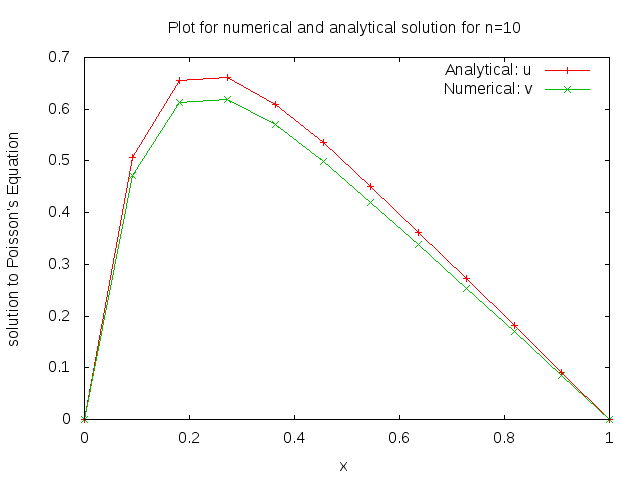
\includegraphics[width=120mm]{Ten.png}
\caption{This shows the numerical and analytical solutions for n =10. The results show that the numerical solution is not very accurate. \label{overflow}}
\end{figure}
\begin{figure}[H]
\centering
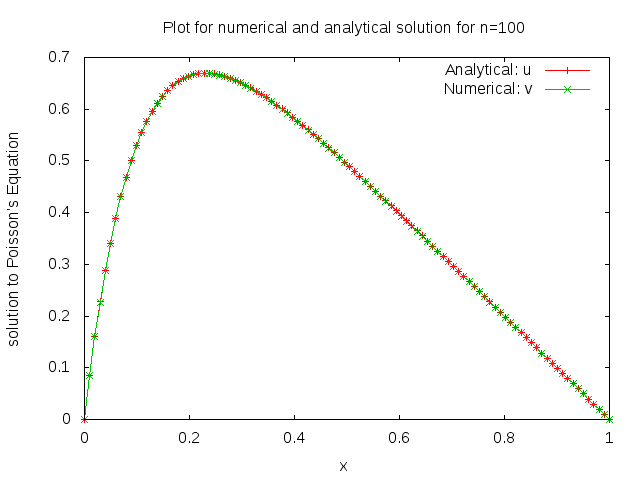
\includegraphics[width=120mm]{Hundred.png}
\caption{This shows the numerical and analytical solutions for n =100. The results show that the numerical solution is more accurate. \label{overflow}}
\end{figure}
\begin{figure}[H]
\centering
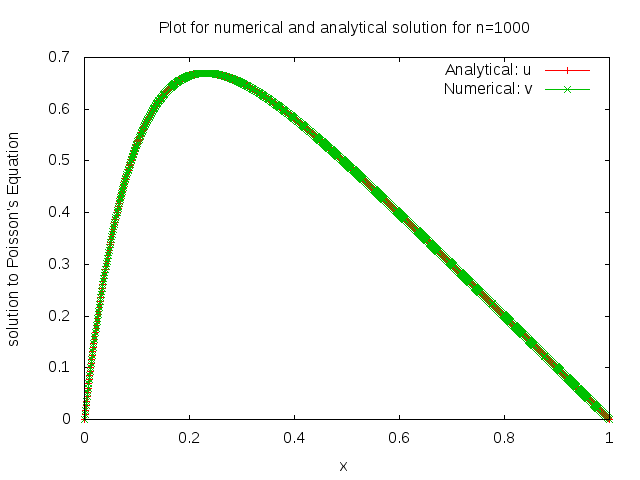
\includegraphics[width=120mm]{Thousand.png}
\caption{This shows the numerical and analytical solutions for n =1000. The results show that the numerical solution very accurate. \label{overflow}}
\end{figure}
\begin{figure}[H]
\centering
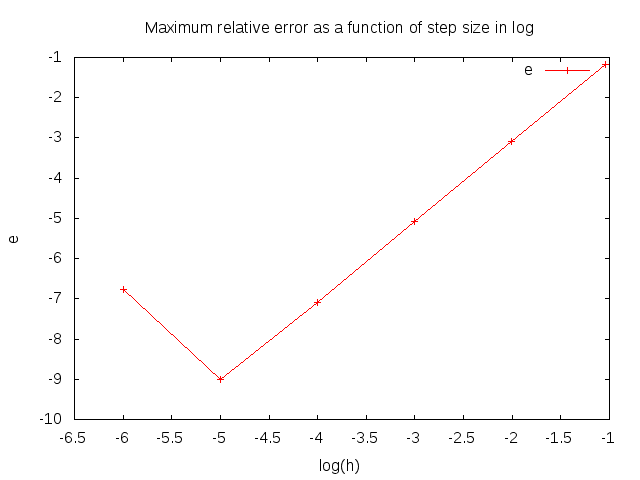
\includegraphics[width=120mm]{log.png}
\caption{This shows the relative error as a function of step size. \label{overflow}}
\end{figure}


\begin{table}[H]
\centering
\label{my-label}
\begin{tabular}{|l|l|l|}
 \cline{1-3}
 Number of grid points, n&  Log of step size, $\log_{10}(h)$ &  Relative error $\epsilon_i$   \\ \cline{1-3}
 $10^1$&  -1.0413927&    -1.1796978\\ \cline{1-3}
 $10^2$&  -2.0043214&    -3.0880368\\ \cline{1-3}
 $10^3$&  -3.0004341&     -5.0800516\\ \cline{1-3}
 $10^4$&  -4.0000434&    -7.0792852\\ \cline{1-3}
 $10^5$&  -5.0000043&    -9.0047052\\ \cline{1-3}
 $10^6$&  -6.0000004&     -6.7713552\\ \cline{1-3}
\end{tabular}
\caption{Values of the maximum relative error with step size in log. }
\end{table}

\begin{table}[H]
\centering
\label{my-label}
\begin{tabular}{|l|l|l|}
 \cline{1-3}
 Number of grid points, n&  Calculation time for tridiagonal method[s]&  Calculation time for LU[s]  \\ \cline{1-3}
 $10^1$&  $9.99\times10^-7$&   $6.79\times10^-5$\\ \cline{1-3}
 $10^2$&  $3.99\times10^-6$&   $3.53\times10^-4$\\ \cline{1-3}
 $10^3$&  $3.19\times10^-5$&   $3.73\times10^-2$\\ \cline{1-3}
 $5000$&  $1.91\times10^-4$&   $8.25\times10^-1$\\ \cline{1-3}
 $10^5$&  $3.88\times10^-4$&    3.70\\ \cline{1-3}
 $10^6$&  $3.20\times10^-2$&     --\\ \cline{1-3}
\end{tabular}
\caption{Values of the computational times.}
\end{table}

\section{Discussion}
Method 1 worked as I expected, the results are shown in Figures 1, 2, and 3. As the step size increased(n) the value improved until 
I go to $n=10^6$ where the relative error started to increase as shown in Table 1. Figure 1(n=10) shows that the step size underestimates the value of the solution and so this is not a good step size. Figures 2 and 3 show that the step size for 100 and 1000 respectively are better. Additionally from Figure 4 I see a slope of 2 from $n=10^5-10$ which is what is expected from the three point formula with $\mathcal{O}(h^2)$. From this figure you can also see where the approximation begins to fail which occurs after $n^5$. After this point the numerical and analytical solutions are so close together that the computer misrepresents the value of the subtraction. As the value of step size gets bigger there is a loss of precision so any step size past $n=10^5$ will deviate from the analytical. 

The main result which I was after was the computational time which is given in table 2. From counting the Floating Point Operations (FLOP) I expected that method 1 would be faster than method 2. The results from table 2 confirm this. For n=10 there is a factor $10^2 $ difference and for $n=10^5$ there is a factor of $10^4$ difference. After this, step size for the LU decomposition becomes impractical since it takes up too much time and memory. I could not implement LU decomposition for $n=10^6$ since the computer gave me an error.

\section{Conclusion}
Solving Poisson's equation with the simplified Gaussian elimination (method 1) was more efficient than with the LU decomposition method(method 2). This was seen by the amount of time it took for the calculation since both gave the same values. Method (2) becomes impractical for large step size and as shown in Table 2, method 1 still works for large numbers but it will also get to the point were the operation takes up too much memory. So by using a simplified Gaussian elimination I was able to perform very efficient calculations by simplifying the main algorithm.

\section{References}
[1] M. Hjorth-Jensen. Computational Physics, Lecture Notes Spring 2016. 

\section{Code Attachment}
\lstinputlisting[language =C++]{"/home/quetzalcoatl/Computational_Physics_work/Project1/Code/Project1.cpp"}

\end{document}

